\documentclass[tikz,border=5pt]{standalone}
\usepackage{luatexja}
\usepackage[hiragino-pron]{luatexja-preset}
\usepackage{amsmath,amssymb}
\usepackage{pgfplots}
\pgfplotsset{compat=1.18}
\usetikzlibrary{arrows.meta,calc,decorations.markings,patterns,positioning}

% Common styles
\tikzset{
  axis/.style={-{Stealth[length=6pt]}, thick},
  curve/.style={thick, red},
  dashed curve/.style={thick, dashed, blue},
  dot/.style={circle, fill, inner sep=1.5pt},
  open dot/.style={circle, draw, fill=white, inner sep=1.5pt},
}

\begin{document}
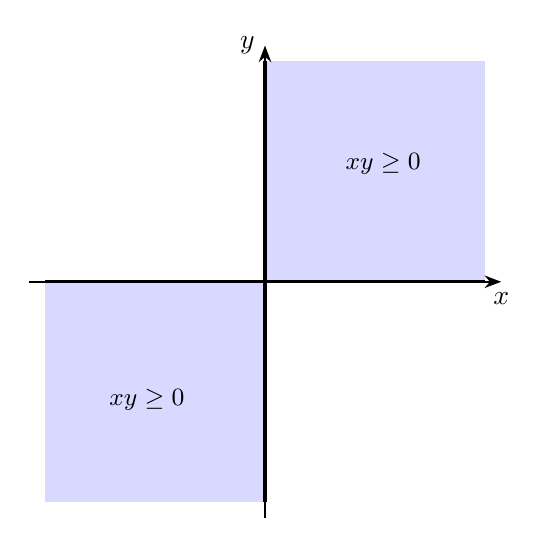
\begin{tikzpicture}
  % Axes
  \draw[axis] (-3,0) -- (3,0) node[below] {$x$};
  \draw[axis] (0,-3) -- (0,3) node[left] {$y$};

  % First quadrant
  \fill[blue, opacity=0.15] (0,0) rectangle (2.8,2.8);

  % Third quadrant
  \fill[blue, opacity=0.15] (0,0) rectangle (-2.8,-2.8);

  % Axes included in domain (very thick, black)
  \draw[very thick] (0,0) -- (2.8,0);
  \draw[very thick] (0,0) -- (0,2.8);
  \draw[very thick] (0,0) -- (-2.8,0);
  \draw[very thick] (0,0) -- (0,-2.8);

  % Label
  \node[font=\small] at (1.5,1.5) {$xy \geq 0$};
  \node[font=\small] at (-1.5,-1.5) {$xy \geq 0$};
\end{tikzpicture}
\end{document}
